\documentclass{article}

\usepackage{blindtext}
\usepackage{graphicx}
\usepackage{caption}
\usepackage{subcaption}
\usepackage{float}
\usepackage[toc,page]{appendix}
\usepackage[margin=0.5in]{geometry}

\restylefloat{figure}

\graphicspath{ {./images/} }



\author{201368087}
\date{\today}
\title{Image Caption Generation}


\begin{document}
    \maketitle
    \tableofcontents

    \section{Text Preparation}
    One of the consequences of lemmatizing the words, means that any suffixes are removed from the words. This allows the model to focus on recognising objects within the image, and describing the object. Whereas without lemmatization, the model will have to also take into the account complex linguistical properties such as grammar, which is hard to model efficiently. Having to do two complex functions within one set of model and weights can be tricky, lemmatization can help to overcome that. Requiring the model to learn both grammar, and describing the image might go against abstraction principle; why should the model be required to do both tasks? It would make more sense for the model to just learn how to caption, and another program, possibly another model, could fix any grammatical mistakes. Especially since lemmatization is a very complex task, as it's not as simple as adding a suffix; in the case of words such as 'good' there is no 'gooder', as one example. Also, lemmatization keeps the vocabulary short, meaning that the model doesn't require to learn how each word can be used, and in which context. Mainly, the advantage of lemmatization is that it focusses the model's attention on relationship between words.\\
    
    However, there are certain issues with lemmatization, as the generated captions will make often no grammatical sense, thus making it harder to evaluate, as there is no simple way to make the sentence be grammatically correct. However, leaving the sentence with grammatical errors, whilst achieving the goal of being close to the original captions, loses in terms of building coherent sentences a human would make. This makes it hard to say whether the model was successful or not. Also, at times lemmatization does not always lead to better performance, therefore it is best to not use it, unless the model's performance cannot be improved, thus trying lemmatization could help the performance. Furthermore, some sentiment analysis tools differentiatte between different words based on the context and give a rating based on the context, thus lemmatization would be harmful if it were to be used in conjunction with tools like VADER.\\
    
    To conclude, lemmatization could remove some useful words, or it could remove a lot of clutter thus leading to a better model. It is hard to say what impact lemmatization would have on the model, without trying it.

    \section{Network Outputs}

    \subsection{LSTM}
    \begin{figure}[H]
        \centering
        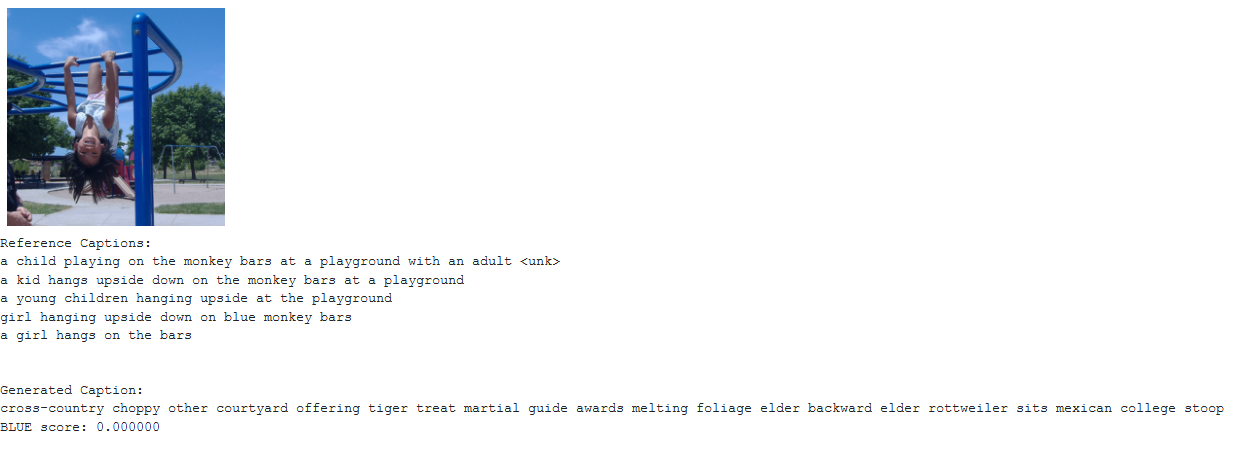
\includegraphics[width=1\textwidth]{lstm_girl_epoch_0.PNG}
        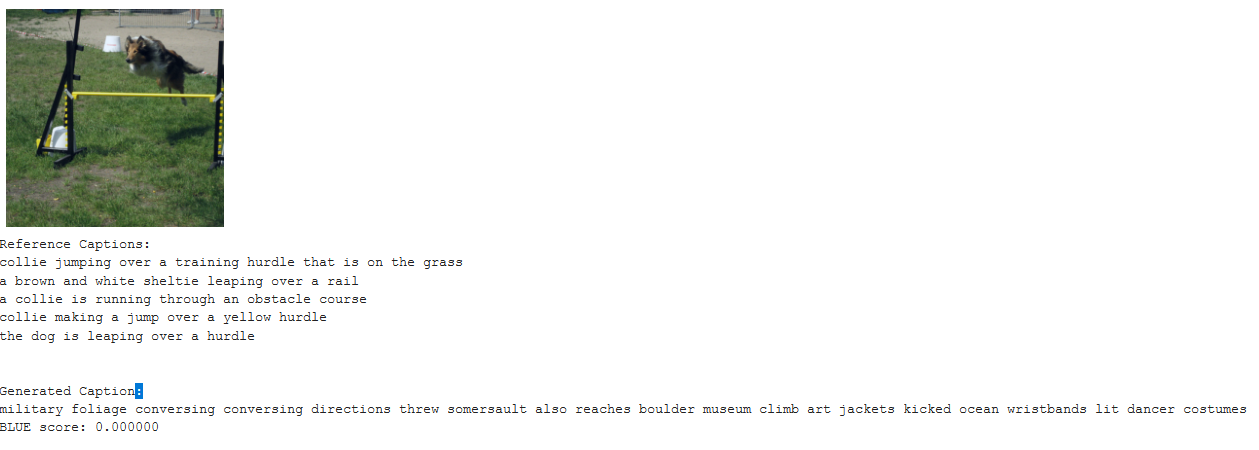
\includegraphics[width=1\textwidth]{lstm_dog_epoch_0.PNG}
        \caption{Initial Caption}
    \end{figure}

    \begin{figure}[H]
        \centering
        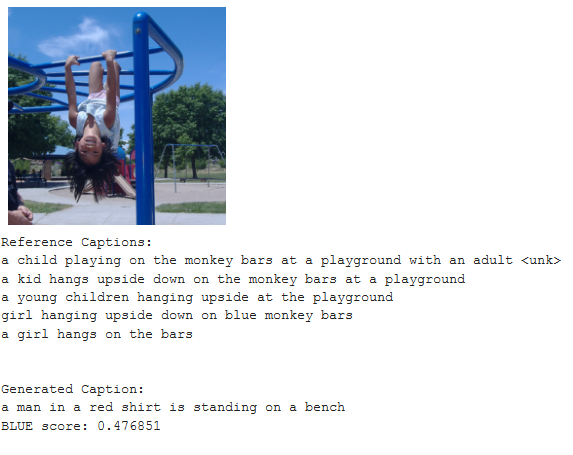
\includegraphics[width=0.4\textwidth]{lstm_girl_epoch_1.PNG}
        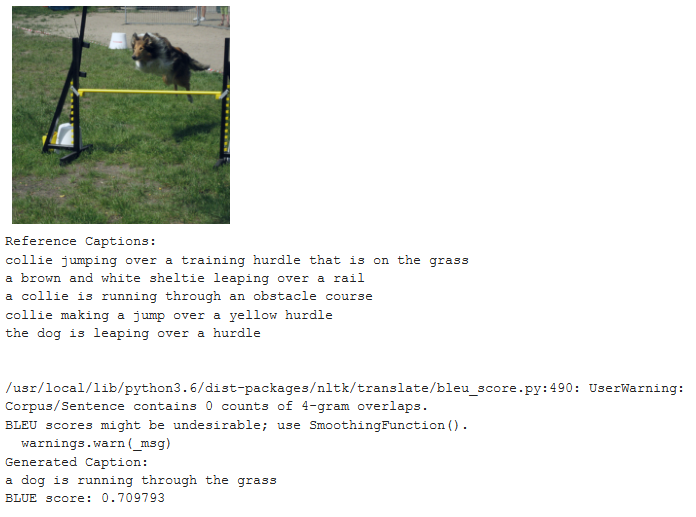
\includegraphics[width=0.4\textwidth]{lstm_dog_epoch_1.PNG}
        \caption{After 1 Epoch}
    \end{figure}

    \begin{figure}[H]
        \centering
        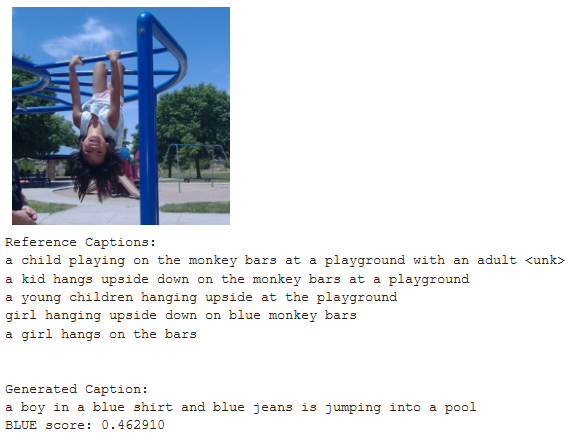
\includegraphics[width=0.4\textwidth]{lstm_girl_epoch_2.PNG}
        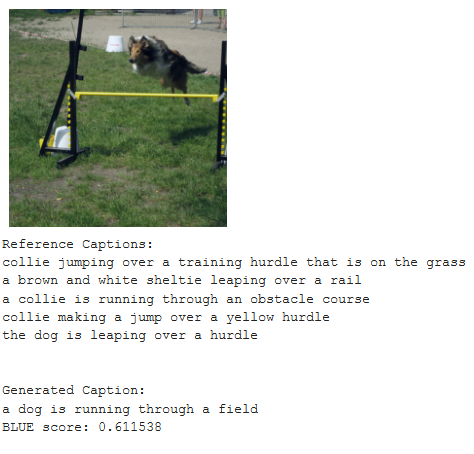
\includegraphics[width=0.35\textwidth]{lstm_dog_epoch_2.PNG}
        \caption{After 2 Epoch}
    \end{figure}

    \begin{figure}[H]
        \centering
        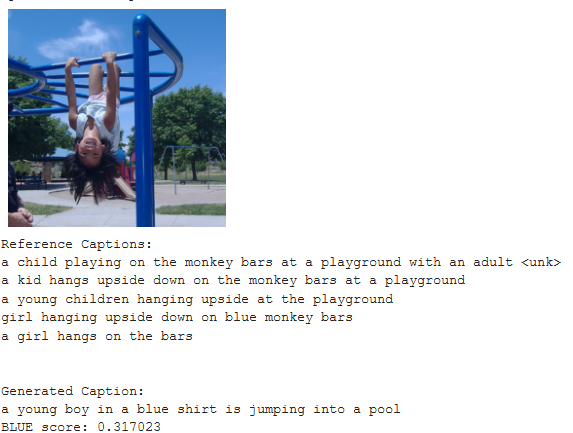
\includegraphics[width=0.4\textwidth]{lstm_girl_epoch_3.PNG}
        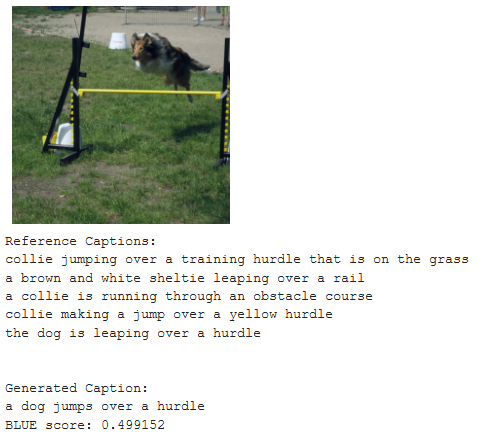
\includegraphics[width=0.35\textwidth]{lstm_dog_epoch_3.PNG}
        \caption{After 3 Epoch}
    \end{figure}

    \begin{figure}[H]
        \centering
        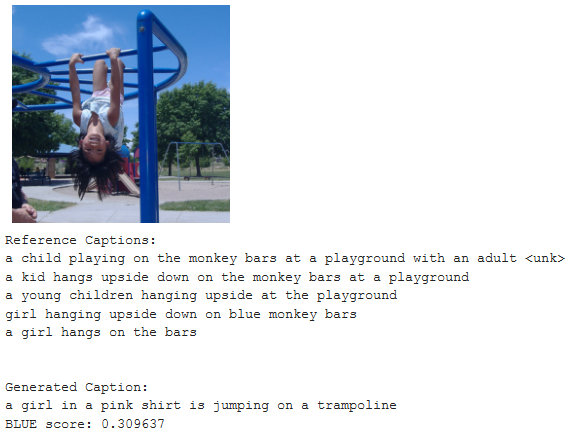
\includegraphics[width=0.4\textwidth]{lstm_girl_epoch_4.PNG}
        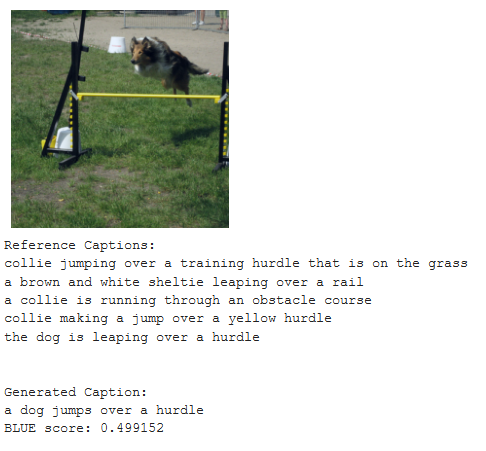
\includegraphics[width=0.35\textwidth]{lstm_dog_epoch_4.PNG}
        \caption{After 4 Epoch}
    \end{figure}

    \begin{figure}[H]
        \centering
        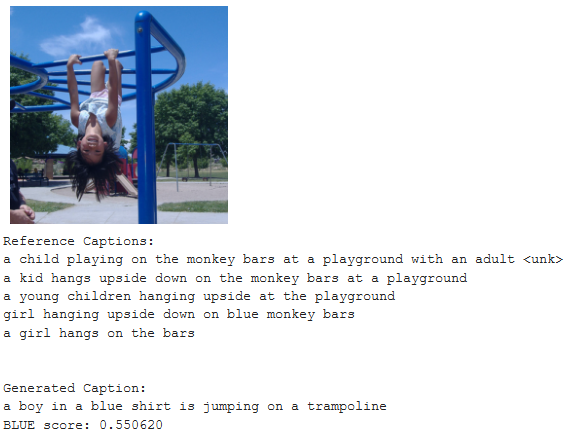
\includegraphics[width=0.4\textwidth]{lstm_girl_epoch_5.PNG}
        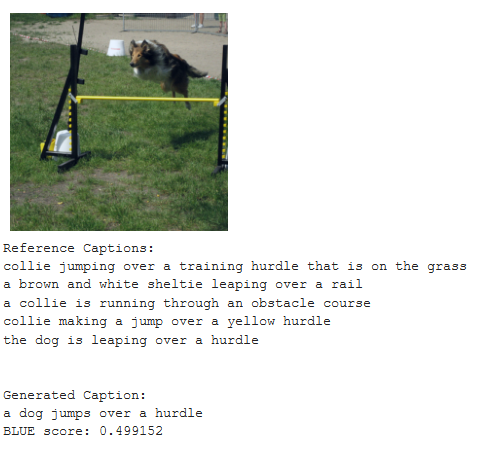
\includegraphics[width=0.35\textwidth]{lstm_dog_epoch_5.PNG}
        \caption{After 5 Epoch}
    \end{figure}

    \subsection{RNN}
    \begin{figure}[H]
        \centering
        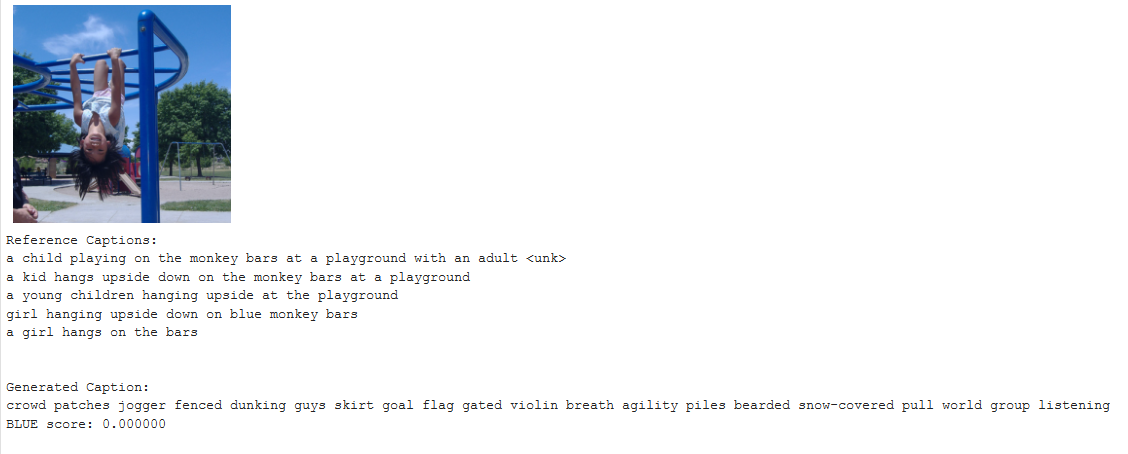
\includegraphics[width=1\textwidth]{rnn_girl_epoch_0.PNG}
        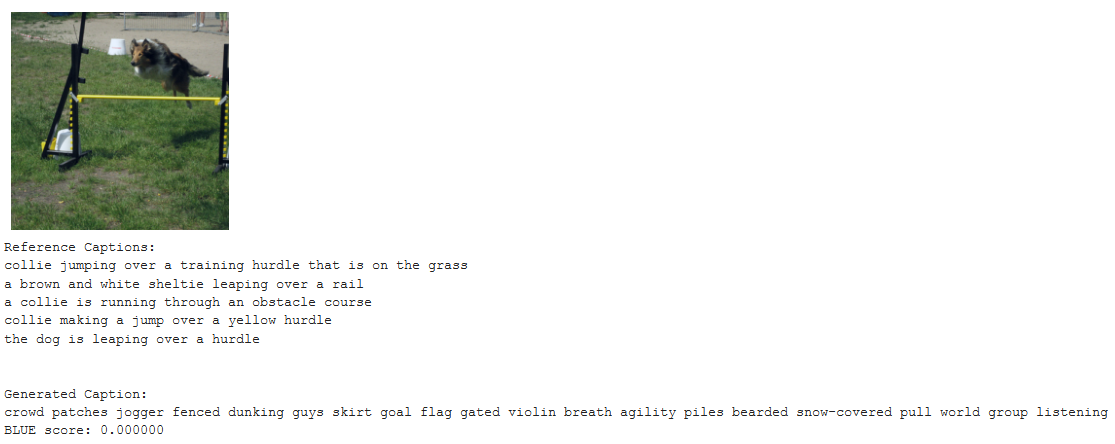
\includegraphics[width=1\textwidth]{rnn_dog_epoch_0.PNG}
        \caption{Initial Caption}
    \end{figure}

    \begin{figure}[H]
        \centering
        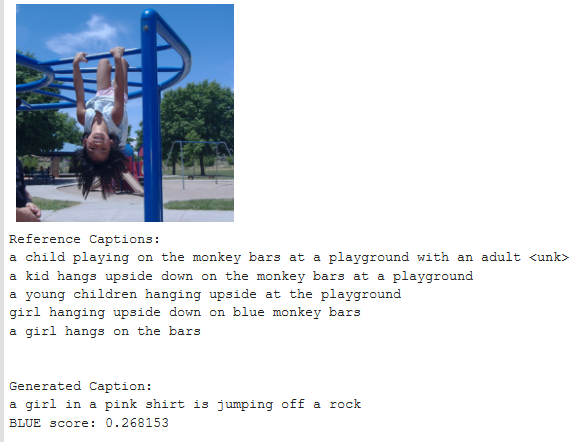
\includegraphics[width=0.4\textwidth]{rnn_girl_epoch_1.PNG}
        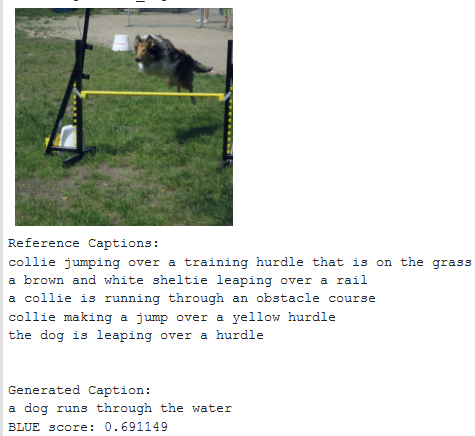
\includegraphics[width=0.35\textwidth]{rnn_dog_epoch_1.PNG}
        \caption{After 1 Epoch}
    \end{figure}

    \begin{figure}[H]
        \centering
        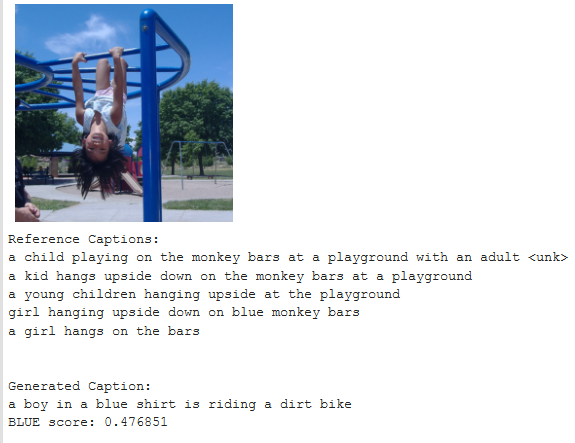
\includegraphics[width=0.4\textwidth]{rnn_girl_epoch_2.PNG}
        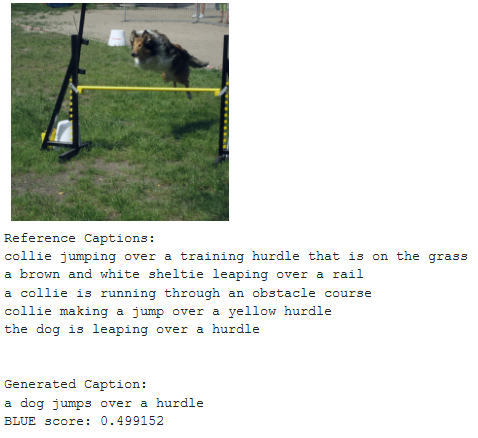
\includegraphics[width=0.35\textwidth]{rnn_dog_epoch_2.PNG}
        \caption{After 2 Epoch}
    \end{figure}

    \begin{figure}[H]
        \centering
        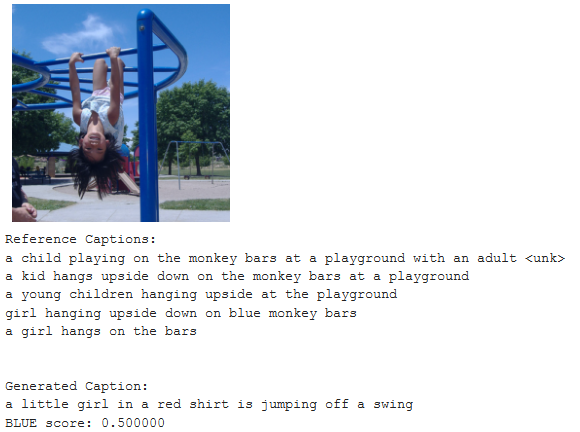
\includegraphics[width=0.4\textwidth]{rnn_girl_epoch_3.PNG}
        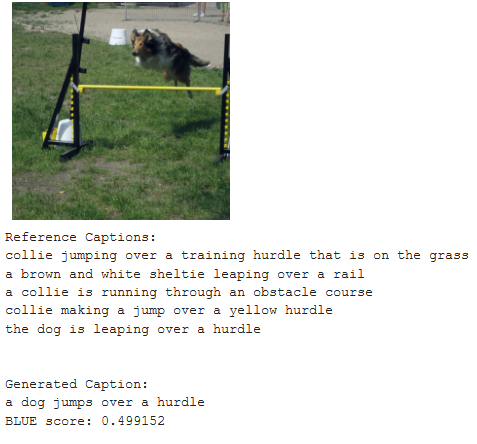
\includegraphics[width=0.35\textwidth]{rnn_dog_epoch_3.PNG}
        \caption{After 3 Epoch}
    \end{figure}

    \begin{figure}[H]
        \centering
        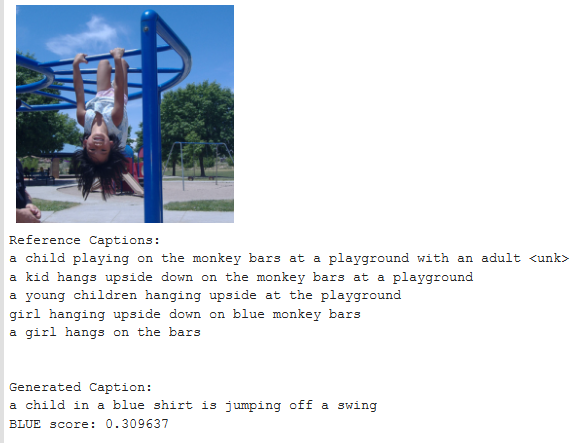
\includegraphics[width=0.4\textwidth]{rnn_girl_epoch_4.PNG}
        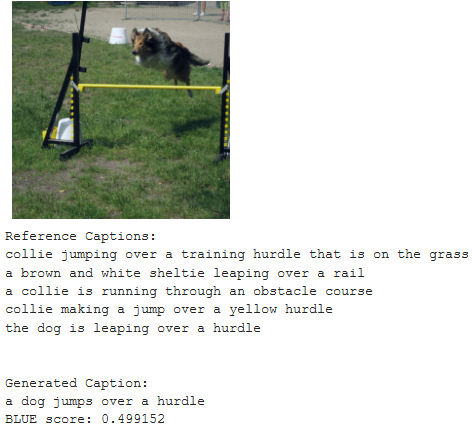
\includegraphics[width=0.35\textwidth]{rnn_dog_epoch_4.PNG}
        \caption{After 4 Epoch}
    \end{figure}

    \begin{figure}[H]
        \centering
        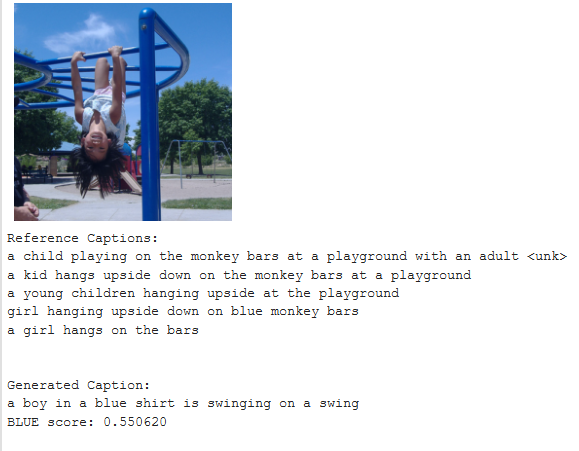
\includegraphics[width=0.4\textwidth]{rnn_girl_epoch_5.PNG}
        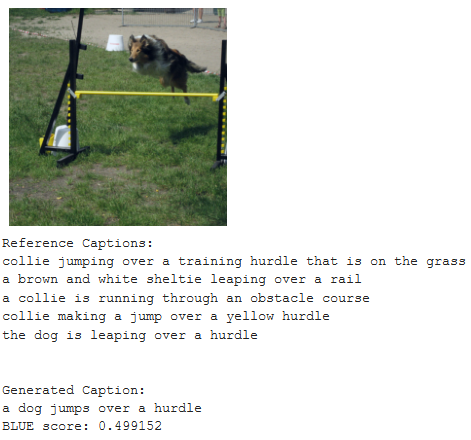
\includegraphics[width=0.35\textwidth]{rnn_dog_epoch_5.PNG}
        \caption{After 5 Epoch}
    \end{figure}


    \section{Comparison of RNN vs LSTM}
    \begin{figure}[h!]
        \centering
        \begin{subfigure}[t]{0.4\textwidth}
            \centering
            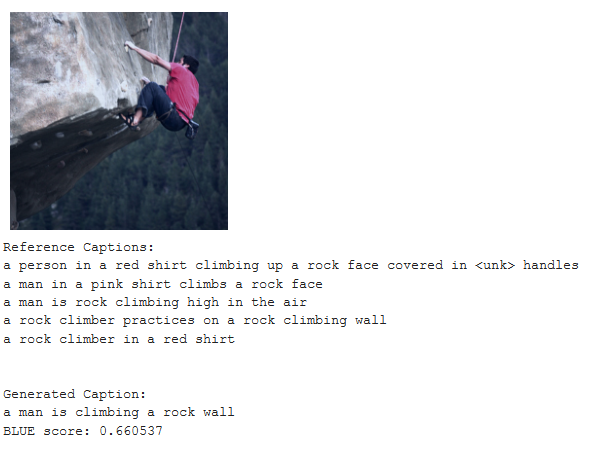
\includegraphics[width=1\textwidth]{climb_lstm.PNG}
            \caption{LSTM}
            \label{figc:figa}
        \end{subfigure}
        \begin{subfigure}[t]{0.4\textwidth}
            \centering
            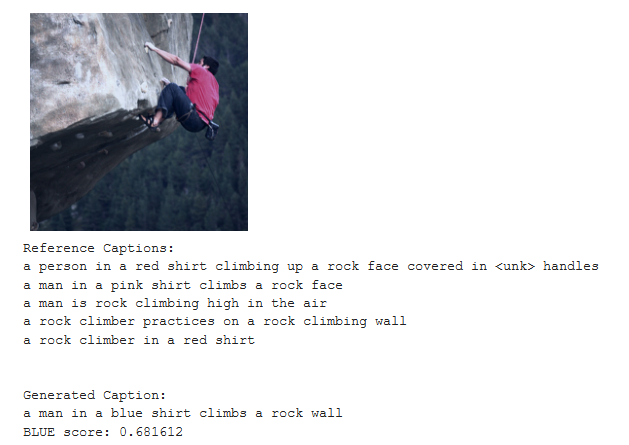
\includegraphics[width=1\textwidth]{climb_rnn.PNG}
            \caption{RNN}
            \label{figc:figb}
        \end{subfigure}
        \caption{Caption of a rock climbing image}
        \label{figc}
    \end{figure}

    \newpage


    \begin{figure}[h!]
        \centering
        \begin{subfigure}[t]{0.4\textwidth}
            \centering
            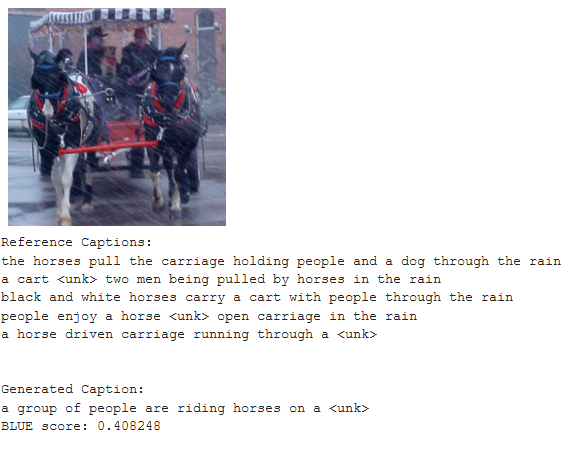
\includegraphics[width=1\textwidth]{lstm_horse.PNG}
            \caption{LSTM}
            \label{figc:figa}
        \end{subfigure}
        \begin{subfigure}[t]{0.4\textwidth}
            \centering
            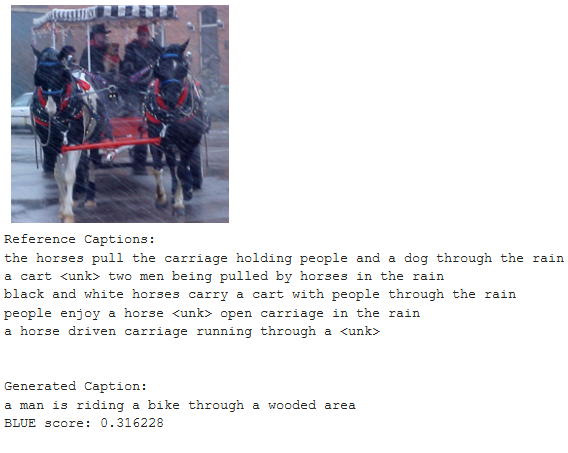
\includegraphics[width=1\textwidth]{rnn_horse.PNG}
            \caption{RNN}
            \label{figc:figb}
        \end{subfigure}
        \caption{Caption of a carriage image}
        \label{figd}
    \end{figure}

    \begin{figure}[h!]
        \centering
        \begin{subfigure}[t]{0.4\textwidth}
            \centering
            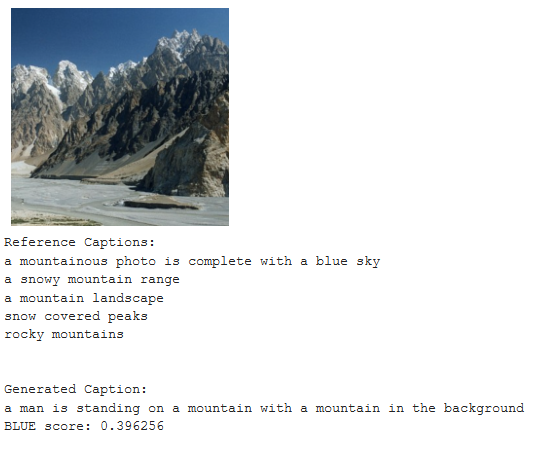
\includegraphics[width=0.75\textwidth]{lstm_mountain.PNG}
            \caption{LSTM}
            \label{figc:figa}
        \end{subfigure}
        \begin{subfigure}[t]{0.4\textwidth}
            \centering
            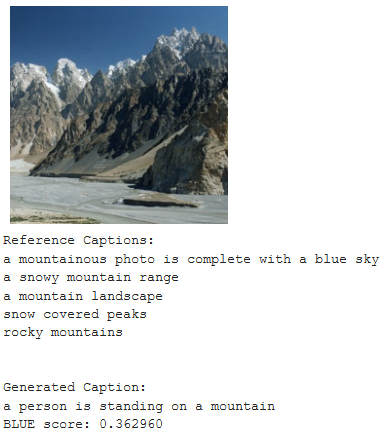
\includegraphics[width=0.55\textwidth]{rnn_mountain.PNG}
            \caption{RNN}
            \label{figc:figb}
        \end{subfigure}
        \caption{Caption of a mountain image}
        \label{fige}
    \end{figure}

    %LOSS
    Firstly, analysing the loss for both the RNN and LSTM, it was between 2.9 and 2.1, and seemed to oscillate around that range, with the RNN ending at 2.5, and LSTM at 2.2. At first, both of the models obviously started high at around 8, which at the end of the first epoch went down to 3.0. After that, it seemed to go up and down at around 2.9-2.1 for both models. However, the RNN would have more variance within epochs. For example, the highest loss for epoch 5 of RNN was 2.5363 whilst lowest one was 2.1525, which is a large difference in this context. This is further magnified by the fact that the LSTM model's fifth epoch ranged between 2.1670 and 2.3768. This trend can be seen in other epochs but slightly less extreme. Considering everything, the loss between the two models is very close, and you would be nitpicking to find any major differences. What the loss boils down to is both the models were consistently improving the loss for the first epoch, and afterwards the loss stagnated and oscillated between a range of values, rather than uniformly decreasing. Conclusively, both of the models struggle in calculating the loss, which is to be expected given that evaluating captions is no easy task. Finally, the time it took to train both models were close and generally, I didn't notice that much of a difference, however it seemed like the RNN took slightly longer.\\
    
    %QUALITY 
    Currently, a more pragmatic approach would be beneficial by looking at the quality of the captions in a less algorithmic way. Personally, a lot of the captions have grammatical structure that would pass by a sentence made by a human. A lot of the captions also accurately depict what is displayed in the image. As an example, the dog image was captioned pretty much spot on. The only issue with it, is the lack of detail. The reference captions often include more detail, such as a breed of a dog, shirt colour of a person, and so on. This goes against what both of the models are outputting, as they seem to be opposed to putting in more detail. This might be due to a lack of reference captions. If all of the reference captions put in detail,  but they do so differently, the model might not recognise that as important, which it arguably isn't. Detail is given so that an object is easier for humans to imagine, contriving the captions from that create a less imaginable image, but yet it's detailed enough to create a basic version, which is one of the main aims of captions. However, captions are also useful for people with blindness or any other health issues targeting vision, thus detail is somewhat required to be able to imagine the image close to what it actually is. Therefore, I struggle to fairly quantify how well the model did in generating captions, as one would expect slightly more detail given.\\ 

    Generally speaking, I would say that the LSTM generally made less mistakes in terms of actually describing the image. However, often, the RNN would try to put detail in, although often incorrect detail. LSTM showed that it could possibly detect the objects better, and give a more accurate yet shallow captions. This can be seen in figure \ref{figc} and especially in the figure \ref{figd}. In figure \ref{figd}, it is clear that the RNN wasn't even close to captioning the image correctly. Both the images also highlight the issue with BLEU scores.\\
    
    %BLEU SCORES
    Furthermore, given the images in the RNN gave a more descriptive caption, however an erroneous one as the person in question does not have a blue shirt. On the other hand, the LSTM managed to give a 100\% correct caption, but much shorter with less detail. However, the BLEU score favours the inaccurate, yet more advanced caption given by the RNN. This shows that the BLEU scores are not perfect, as, personally, the less descriptive but accurate statement should be scored way higher given that it is completely plausible that a human would give such a caption. Generally, the models don't favour descriptive captions. This is reinforced by the fact that in both the RNN and LSTM flavours, the 'a dog jumps over the hurdle' caption doesn't change for 3 epochs.\\

    In general, I have found out that the BLEU scores can be quite misleading in certain cases. This is due to the fact that the BLUE scores strictly calculates how close it is to the reference captions, thus leading to some confusing scores. For example, for the dog image the caption 'a dog jumps over a hurdle' gets a lower score than 'a dog runs through water'. This is partly due to the weights I have chosen for the n-grams. I have decided to use $weights=(0.5, 0.25, 0.15, 0.1)$, as I did not want to put too much emphasis on the 3/4-gram as in my testing, 'a dog jumps over a hurdle' would get an even lower score. The consequence of that though is that the BLEU score favour captions that contain specific words like 'running' more so than a combination of particular words. However, looking in the future, I believe this would be more beneficial as relying on a high 4-gram might make the model use only one specific sentence structure, making the captions more monotonous and less human-like. Furthermore, 4-grams may reduce the amount of adjectives used, as 4-gram relies on the adjectives being stagnant.\\

    %LONG VS SHORT
    One of the main issues with both the models is that they struggle when the captions get large in size. Generally speaking, when a caption is short, both the models seem to do an adequate job, with the LSTM being close to perfect. However, when the image is slightly more complex, both of the models struggle, which again can be seen in the figures above. Strangely enough, both the models struggle when the reference caption put too little detail in, as seen in figure \ref{fige}.\\

    To conclude, the LSTM model seemed to generally perform slightly better to the RNN, and often identify the right object. The main issue for both models seemed to be getting captions with the right amount of balance between detail and succinctness, both to train on and to generate.



    \section{Additional Text Annotation Files}

    There are two files; namely ExpertAnnotations.txt and CrowdFlowerAnnotations.txt. ExpertAnnotations.txt contains a table of images and captions from other images, which the expert ranked from 1-4 as to whether a caption from that different image is similar to the image in question. In similar vein, the CrowdFlowerAnnotations.txt file contains the number of yeses and number of noes whether a caption from a different image describes another image. A percentage of yesses is also recorded.\\

    These files have similar functions, which solve a hard problem when it comes to models in this domain, which is encapsulating the wide variety of ways to describe a given image. There is no one fixed solution to the problem, and there are countless ways to describe an image that are perfectly fine, or at least convey the basic message. Even if the model manages to successfully come close to the captions used in training, there are other ways that describe the image just as well, but with different level of detail or tone etc. Thus, the hardest part would be to get a large sample size to effectively narrow down a way of describing that object. Trying to encapsulate all the possible ways gets even harder when you consider words that portray different emotions like 'badly' or 'awesome'. Furthermore, the amount of detail given may wary from person to person, as seen previously with \textit{figure \ref{figc}}. Such variance is proven to be tricky to evaluate, thus to improve confidence of the model, it might be more beneficial to define what not to do, rather than what to do.\\ 

    These files would help with this issue, as they could be used as a similarity ranking between the different forms of captions. The files can also be used in a unique way comparatively to the captions attached to the images, as they can show which captions they shouldn't be close to. For example, if a caption is close in nature to a caption with a lot of 'No's given by the experts/crowd then that can be considered an inadequate caption and possibly count it in the loss function. This also gives a better way to evaluate the model, as if the caption is somewhat close to the attached captions, but close to captions it shouldn't be close to, then it might suggest that the model still hasn't fully recognised the object in question, and a lot of the score can be attributed to containing stop words like 'the'.


    % - an understanding of the contents of those two text files
    % - an understanding of a key problem in this domain and how those additional files can help address the problem
    % - your idea, justified, of how they could be incorporated into the model training and evaluation 

    % \bibliographystyle{abbrv}
    % \bibliography{ref}
\end{document}